\documentclass[11pt,a4paper]{article}

\usepackage[margin=2.2cm]{geometry}
\usepackage{xcolor}
\usepackage{tikz}
\usetikzlibrary{arrows.meta,positioning,shapes.geometric,fit,backgrounds,shadows,calc}
\usepackage{booktabs}
\usepackage{longtable}
\usepackage{array}
\usepackage{enumitem}
\usepackage{titlesec}
\usepackage{fancyhdr}
\usepackage{hyperref}
\usepackage{listings}
\usepackage{parskip}
\usepackage{tcolorbox}
\tcbuselibrary{skins,breakable}

% ---------- colours ----------
\definecolor{ink}{HTML}{1a1a2e}
\definecolor{accent}{HTML}{5b5bd6}
\definecolor{accent2}{HTML}{16a085}
\definecolor{warn}{HTML}{d97706}
\definecolor{danger}{HTML}{c0392b}
\definecolor{soft}{HTML}{f4f4fb}
\definecolor{codebg}{HTML}{f6f6f9}

\hypersetup{
  colorlinks=true,
  linkcolor=accent,
  urlcolor=accent2,
  citecolor=accent,
  pdftitle={TruCart -- Project Report},
  pdfauthor={Bhautik Vaghamshi, Daksh Patel}
}

\titleformat{\section}{\Large\bfseries\color{ink}}{\thesection}{0.5em}{}[{\color{accent}\titlerule[1.2pt]}]
\titleformat{\subsection}{\large\bfseries\color{ink}}{\thesubsection}{0.5em}{}
\titleformat{\subsubsection}{\normalsize\bfseries\color{accent}}{\thesubsubsection}{0.5em}{}

\pagestyle{fancy}
\fancyhf{}
\renewcommand{\headrulewidth}{0.4pt}
\fancyhead[L]{\small\textcolor{ink}{TruCart -- Interview Reference}}
\fancyhead[R]{\small\thepage}
\fancyfoot[C]{\small\textcolor{gray}{Autonomous AI Operations Platform}}

\lstdefinestyle{code}{
  basicstyle=\ttfamily\small,
  backgroundcolor=\color{codebg},
  frame=single,
  rulecolor=\color{gray!40},
  breaklines=true,
  columns=fullflexible,
  showstringspaces=false,
  xleftmargin=4pt,
  xrightmargin=4pt,
}
\lstset{style=code}

\newtcolorbox{keybox}[1][]{
  colback=soft, colframe=accent, boxrule=0.6pt, arc=2pt,
  left=6pt, right=6pt, top=4pt, bottom=4pt, breakable, #1
}
\newtcolorbox{qabox}[1]{
  colback=white, colframe=accent!60, boxrule=0.5pt, arc=2pt,
  left=6pt, right=6pt, top=5pt, bottom=5pt, breakable,
  title={#1}, fonttitle=\bfseries\color{ink}, coltitle=ink,
  colbacktitle=soft
}

\newcommand{\Rs}{Rs.\,}
\newcommand{\agenthead}[2]{%
  \subsection*{\textcolor{accent}{#1}}%
  \textit{#2}\par\vspace{2pt}
}

\title{
  \vspace{-1.5cm}
  {\Huge\bfseries\color{ink} TruCart}\\[6pt]
  {\Large AI-Assisted E-Commerce Operations Platform}\\[4pt]
  {\large\color{gray} Full Project Report -- Architecture, Agents, APIs, Infra \& Interview Notes}
}
\author{Bhautik Vaghamshi \and Daksh Patel \\ \small B.Tech Semester 7 -- Hackathon Build}
\date{\small \today}

\begin{document}
\maketitle
\thispagestyle{empty}

\begin{keybox}
\textbf{What this document is.} A complete, plain-language walkthrough of everything that is
actually implemented in the TruCart codebase -- not the future vision, not the pitch deck.
Every section maps to real files in the repository so you can open the code and match it
line-for-line while explaining it to an interviewer. Diagrams are hand-drawn (TikZ) to mirror
the Mermaid diagrams already in \texttt{docs/architecture.md}.
\end{keybox}

\tableofcontents
\newpage

% =====================================================================
\section{The Problem, In One Paragraph}
% =====================================================================

Running an e-commerce store means juggling six back-office jobs at once: watching stock levels,
confirming and shipping orders, answering support tickets, repricing products as costs and
demand shift, running clearance campaigns on overstock, and tracking shipments. Normally a
person (or a team) does each of these jobs by hand, in separate tools, which means decisions
are slow and inconsistent. \textbf{TruCart replaces each of those six jobs with a small,
specialised AI agent} that watches its own slice of the database, makes a bounded decision
(with an LLM as an advisor, never as an unchecked authority), executes the decision itself if
it is low-risk, and pushes it to a human \emph{review queue} if it is not. A scheduler runs
every agent in sequence every few minutes so the store keeps running on its own; a human only
steps in for the judgement calls that matter.

The distinguishing feature -- and the one worth leading with in an interview -- is the
\textbf{Autopilot Ledger}: every autonomous decision is booked against a computed
``what would have happened if we did nothing'' baseline, checked against the real outcome
weeks later, and rolled into a trust score per agent. This turns ``the AI made a decision''
into ``the AI made a decision, and here is the receipt proving whether it was a good one.''

% =====================================================================
\section{System Architecture}
% =====================================================================

TruCart is a small monorepo (npm workspaces + Turborepo) with three real pieces: a Next.js
dashboard, a FastAPI agent service, and a Postgres (Supabase) database. Nothing else is a
separate service -- there is no message queue, no container orchestrator, no external
microservice mesh. Simplicity was a deliberate choice: every piece needed to run for \$0 on
free tiers.

\begin{figure}[h]
\centering
\resizebox{\linewidth}{!}{%
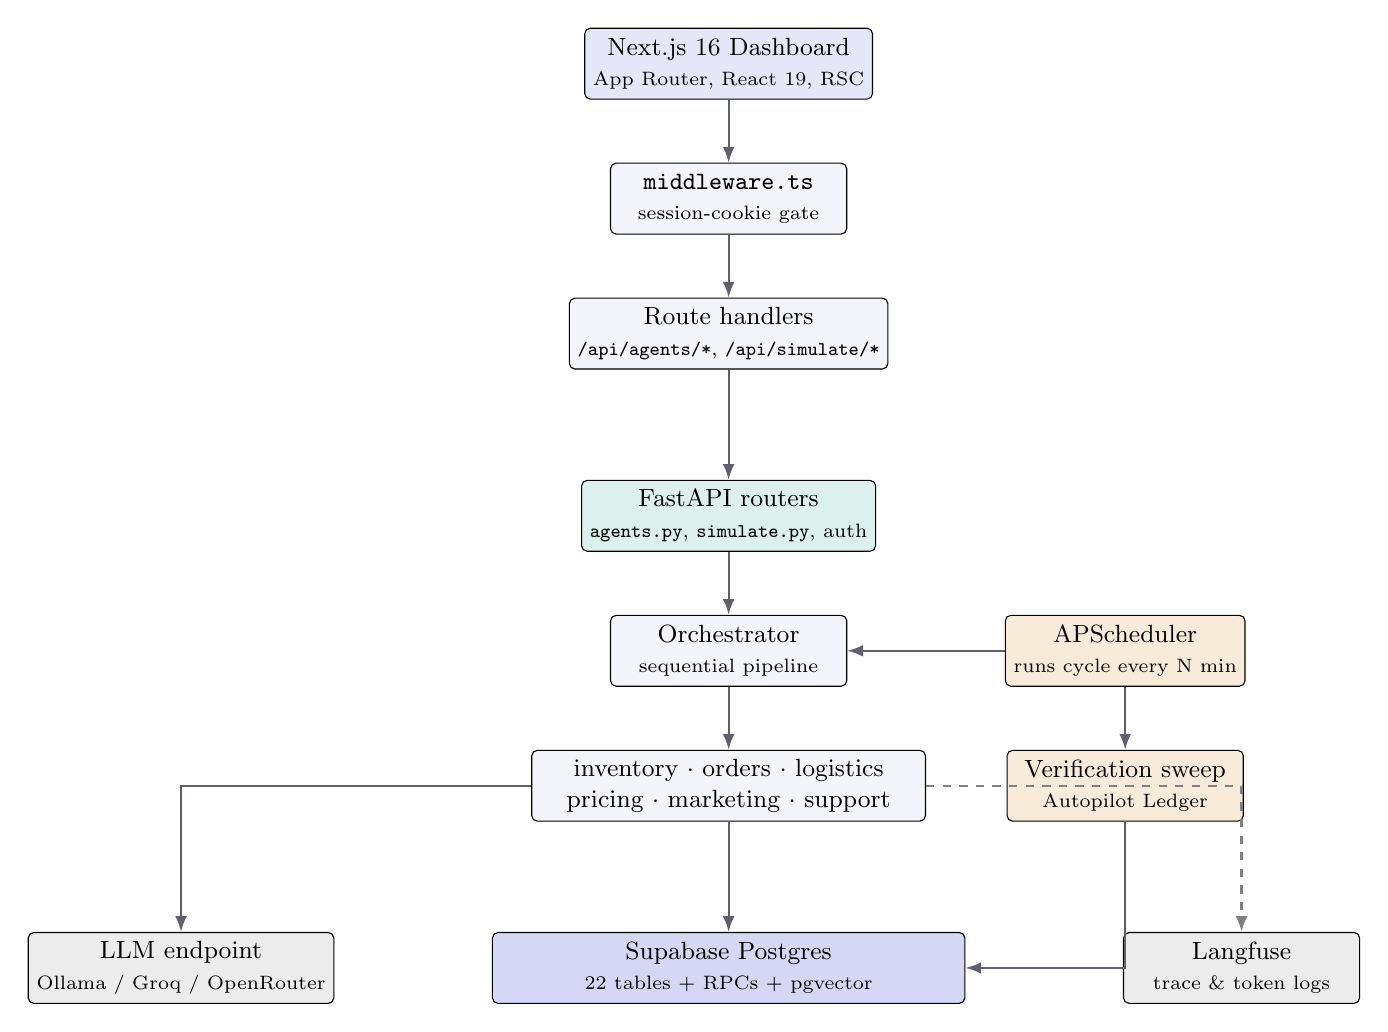
\begin{tikzpicture}[
  node distance=8mm and 20mm,
  box/.style={draw, rounded corners=2pt, fill=soft, minimum height=9mm, minimum width=30mm, align=center, font=\small, inner sep=3pt},
  arr/.style={-{Latex[length=2mm]}, thick, color=ink!70},
  dashedarr/.style={-{Latex[length=2mm]}, thick, dashed, color=gray}
]
% Browser tier
\node[box, fill=accent!15] (ui) {Next.js 16 Dashboard\\ \scriptsize App Router, React 19, RSC};

% Web tier
\node[box, below=of ui] (mw) {\texttt{middleware.ts}\\ \scriptsize session-cookie gate};
\node[box, below=of mw] (proxy) {Route handlers\\ \scriptsize \texttt{/api/agents/*}, \texttt{/api/simulate/*}};

% Agent tier
\node[box, below=14mm of proxy, fill=accent2!15] (routes) {FastAPI routers\\ \scriptsize \texttt{agents.py}, \texttt{simulate.py}, auth};
\node[box, below=of routes] (orch) {Orchestrator\\ \scriptsize sequential pipeline};
\node[box, below=of orch, minimum width=50mm] (agents) {inventory $\cdot$ orders $\cdot$ logistics\\ pricing $\cdot$ marketing $\cdot$ support};
\node[box, right=of orch, fill=warn!15] (sched) {APScheduler\\ \scriptsize runs cycle every N min};
\node[box, below=of sched, fill=warn!15] (sweep) {Verification sweep\\ \scriptsize Autopilot Ledger};

% Data tier
\node[box, below=14mm of agents, fill=accent!25, minimum width=60mm] (pg) {Supabase Postgres\\ \scriptsize 22 tables + RPCs + pgvector};

% External
\node[box, left=20mm of pg, fill=gray!15] (llm) {LLM endpoint\\ \scriptsize Ollama / Groq / OpenRouter};
\node[box, right=20mm of pg, fill=gray!15] (lf) {Langfuse\\ \scriptsize trace \& token logs};

\draw[arr] (ui) -- (mw);
\draw[arr] (mw) -- (proxy);
\draw[arr] (proxy) -- (routes);
\draw[arr] (routes) -- (orch);
\draw[arr] (orch) -- (agents);
\draw[arr] (sched) -- (orch);
\draw[arr] (sched) -- (sweep);
\draw[arr] (agents.south) -- (pg.north);
\draw[arr] (sweep) |- (pg);
\draw[arr] (agents.west) -| (llm.north);
\draw[dashedarr] (agents.east) -| (lf.north);
\end{tikzpicture}%
}
\caption{Three real tiers: browser $\to$ Next.js web tier $\to$ FastAPI agent tier $\to$ Postgres, with an LLM and Langfuse as optional side dependencies.}
\end{figure}

\begin{center}
\begin{tabular}{@{}p{2.4cm}p{6.2cm}p{5.6cm}@{}}
\toprule
\textbf{Layer} & \textbf{Technology} & \textbf{Where it runs} \\
\midrule
Dashboard & Next.js 16 (App Router), React 19, Tailwind v4, \texttt{shadcn/ui} (\texttt{packages/ui}) & Vercel Hobby (or Docker) \\
Web APIs / auth & Next.js route handlers, \texttt{jose} HS256 JWT session cookie & same as above \\
Agents / orchestrator & FastAPI, APScheduler, OpenAI-compatible SDK & Fly.io / Render / EC2 / Docker \\
Database & Supabase Postgres + \texttt{pgvector}, plain SQL migrations (no ORM) & Supabase free tier \\
LLM inference & Local Ollama \texttt{qwen2.5:7b} \emph{or} any OpenAI-compatible free endpoint (Groq, OpenRouter) & self-host or free API \\
Tracing & Langfuse (\texttt{langfuse.openai} drop-in wrapper) & Langfuse Cloud free \\
\bottomrule
\end{tabular}
\end{center}

\subsection{Why this shape}
\begin{itemize}[itemsep=2pt]
  \item \textbf{No ORM.} All 16 migrations are hand-written SQL. This keeps every RPC (stored
  procedure) auditable and lets the team encode business rules (e.g. ``never let a reservation
  exceed stock on hand'') directly in the database as atomic transactions, rather than in
  application code that could race.
  \item \textbf{No message bus.} Agents coordinate purely through shared Postgres state and
  a single \texttt{correlation\_id} per cycle -- see \S\ref{sec:coordination}. This was a
  conscious trade-off: much simpler to reason about and debug than a pub/sub system, at the
  cost of only supporting sequential hand-offs.
  \item \textbf{LLM is advisory, not authoritative.} Every agent calls the LLM for one bounded
  JSON decision (e.g. ``raise, reduce, or hold, and to what price''), then clamps that decision
  with deterministic guardrails written in Python. If the LLM is unreachable, the agent falls
  back to a deterministic rule and keeps working -- the system never breaks because an LLM
  timed out.
\end{itemize}

% =====================================================================
\section{The Six Agents}
% =====================================================================

All agents live in \texttt{backend/agents/} and share one shape: they load their own tunable
knobs from the \texttt{agent\_config} table, scan their slice of the database, optionally ask
the LLM for a judgement call via \texttt{call\_llm\_json(...)}, apply hard guardrails, execute
the safe actions immediately, push the risky ones to \texttt{review\_queue}, write one row to
\texttt{agent\_task\_log}, and emit \texttt{notify(...)} rows that show up as dashboard
notifications.

\begin{figure}[h]
\centering
\resizebox{\linewidth}{!}{%
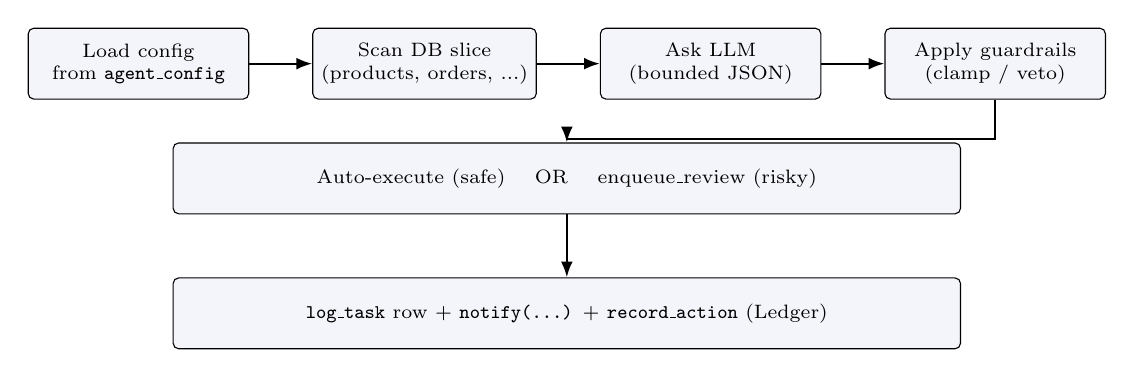
\begin{tikzpicture}[
  node distance=8mm,
  stepbox/.style={draw, rounded corners=2pt, fill=soft, minimum width=28mm, minimum height=9mm, align=center, font=\scriptsize, inner sep=3pt},
  arr/.style={-{Latex[length=2mm]}, thick}
]
\node[stepbox] (a) {Load config\\ from \texttt{agent\_config}};
\node[stepbox, right=8mm of a] (b) {Scan DB slice\\ (products, orders, ...)};
\node[stepbox, right=8mm of b] (c) {Ask LLM\\ (bounded JSON)};
\node[stepbox, right=8mm of c] (d) {Apply guardrails\\ (clamp / veto)};
\node[stepbox, below=10mm of $(a)!0.5!(d)$, minimum width=100mm, xshift=0mm] (e) {Auto-execute (safe) \quad OR \quad enqueue\_review (risky)};
\node[stepbox, below=8mm of e, minimum width=100mm] (f) {\texttt{log\_task} row + \texttt{notify(...)} + \texttt{record\_action} (Ledger)};
\draw[arr] (a) -- (b); \draw[arr] (b) -- (c); \draw[arr] (c) -- (d);
\draw[arr] (d.south) -- ++(0,-5mm) -| (e.north);
\draw[arr] (e) -- (f);
\end{tikzpicture}%
}
\caption{The common shape every agent follows.}
\end{figure}

\agenthead{1. Inventory Agent (\texttt{inventory.py})}{Restocking -- finds products at or below
their reorder point and raises purchase orders.}
\begin{itemize}[itemsep=1pt]
\item Scans \texttt{products} joined with \texttt{inventory} for items where
\texttt{quantity\_on\_hand} $\le$ \texttt{reorder\_point}.
\item Orders a fixed \texttt{reorder\_quantity} (not demand-forecasted in this build -- a
known simplification, see \S\ref{sec:limits}).
\item The LLM writes the human-readable restock justification text only; the reorder decision
itself is rule-based.
\item \textbf{Guardrail:} a PO auto-approves only if its total cost $\le$
\texttt{po\_auto\_approve\_limit} (default \Rs{}5{,}000); otherwise it goes to
\texttt{review\_queue}.
\item \textbf{Receiving:} approved POs are received automatically after
\texttt{receiving\_lead\_days} via the \texttt{receive\_purchase\_order} RPC, which increments
on-hand stock -- so the loop (order $\to$ receive $\to$ stock goes up) is closed, not just the
ordering half.
\end{itemize}

\agenthead{2. Order Agent (\texttt{orders.py})}{Confirms paid orders and reserves stock --
purely mechanical, no LLM.}
\begin{itemize}[itemsep=1pt]
\item Finds \texttt{pending} orders with \texttt{payment\_status = 'paid'}.
\item Calls the \texttt{confirm\_order\_and\_reserve} RPC, an atomic Postgres transaction that
checks stock availability and reserves it in the same statement -- preventing a race where two
concurrent orders both think stock is available.
\item \textbf{Escalates} orders that are unpaid, have no items, or exceed available stock.
\end{itemize}

\agenthead{3. Logistics Agent (\texttt{logistics.py})}{Drives the shipment lifecycle --
purely mechanical, no LLM.}
\begin{itemize}[itemsep=1pt]
\item Creates a shipment for every newly confirmed order (invents a carrier name, tracking
number, and flat shipping cost -- there is no real carrier API).
\item Advances shipments through \texttt{label\_created $\to$ in\_transit $\to$
out\_for\_delivery $\to$ delivered} on a time basis (\texttt{transit\_hours}), not real carrier
webhooks.
\item Flags shipments stuck at one stage too long as exceptions for review.
\end{itemize}

\agenthead{4. Pricing Agent (\texttt{pricing.py})}{The most sophisticated agent -- reprices
products based on our \emph{own} economics, not competitor scraping.}
\begin{itemize}[itemsep=1pt]
\item For every active product it computes: the \textbf{effective unit cost} (from the latest
approved/received purchase order, falling back to \texttt{cost\_price}), the resulting
\textbf{current gross margin}, \textbf{days of stock cover} (on-hand stock $\div$ trailing
90-day daily sales velocity), and days since the last price change.
\item Flags a candidate if margin is \emph{squeezed} below \texttt{min\_margin\_pct}, cost
\emph{rose} enough to threaten the target margin, the product is \emph{overstocked} (cover
$>$ \texttt{overstock\_cover\_days} \emph{and} margin already healthy), or cost \emph{fell}.
\item Sends the top candidates to the LLM with exactly these numbers and asks for
\texttt{raise|reduce|hold}, a target price, urgency, and a one-sentence rationale.
\item \textbf{Guardrails clamp the LLM's answer no matter what it said:} the final price is
capped to $\pm$\texttt{price\_change\_max\_pct} (15\%) of the current price, floored at the
margin that yields \texttt{min\_margin\_pct}, and \textbf{never allowed below unit cost}.
\item \textbf{Escalates} if the move would go below cost, breach the margin floor, or the LLM
marked it \texttt{urgency: high}. Applied through the \texttt{apply\_price\_change} RPC (which
records \texttt{price\_history} and updates \texttt{products.current\_price} atomically).
\end{itemize}

\agenthead{5. Marketing Agent (\texttt{marketing.py})}{Detects overstock and drafts clearance
campaigns.}
\begin{itemize}[itemsep=1pt]
\item Overstock test: \texttt{on\_hand} $>$ \texttt{reorder\_point} $\times$ a multiplier (a
coarse heuristic, not true demand modelling).
\item The LLM writes the campaign subject, body copy, and target segment.
\item \textbf{Guardrail:} auto-activates if the estimated budget $\le$
\texttt{budget\_auto\_approve\_limit}; otherwise goes to review.
\item ``Sending'' a campaign just inserts a \texttt{campaigns} row and fabricated metrics --
there is no real ESP integration.
\item \textbf{Conflict guard:} the orchestrator passes marketing a \texttt{skip\_product\_ids}
set containing every SKU that inventory or pricing already touched \emph{in the same cycle},
so marketing never launches a clearance sale on a product that was simultaneously repriced or
just reordered.
\end{itemize}

\agenthead{6. Support Agent (\texttt{support.py})}{Triages open tickets with retrieval-augmented
generation (RAG).}
\begin{itemize}[itemsep=1pt]
\item Retrieves the customer's order history and, via the \texttt{match\_knowledge\_base}
pgvector RPC, the top relevant policy/FAQ chunks (return policy, refund windows, etc.).
\item The LLM \textbf{chooses the action} -- resolve, refund, or escalate -- with a confidence
score, using the retrieved context.
\item \textbf{Guardrail:} a refund amount is clamped to the order total and auto-approves only
under \texttt{refund\_auto\_approve\_limit} (default \Rs{}100); larger refunds always go
to review. Refunds are whole-order only (no partial refunds / RMA in this build).
\end{itemize}

\subsection{Guardrail thresholds -- where they live}
Two config tables separate ``how does this agent behave'' from ``what dollar amount needs a
human'':
\begin{itemize}[itemsep=1pt]
\item \texttt{store\_config} -- cross-cutting approval ceilings:
\texttt{po\_auto\_approve\_limit}, \texttt{refund\_auto\_approve\_limit},
\texttt{price\_change\_max\_pct}, plus the Ledger's settle-day windows.
\item \texttt{agent\_config} -- per-agent tunables: \texttt{max\_items\_per\_run},
\texttt{min\_margin\_pct}, \texttt{target\_margin\_pct}, \texttt{demand\_window\_days}, etc.
\end{itemize}
Both are editable live from \texttt{/dashboard/agents $\to$ Configure} -- no redeploy needed to
tighten or loosen an agent's autonomy.

% =====================================================================
\section{Multi-Agent Coordination}
\label{sec:coordination}
% =====================================================================

TruCart deliberately does \textbf{not} use a message bus, an event queue, or agent-to-agent
messaging. Coordination is \textbf{sequential + shared database state}:

\begin{figure}[h]
\centering
\resizebox{\linewidth}{!}{%
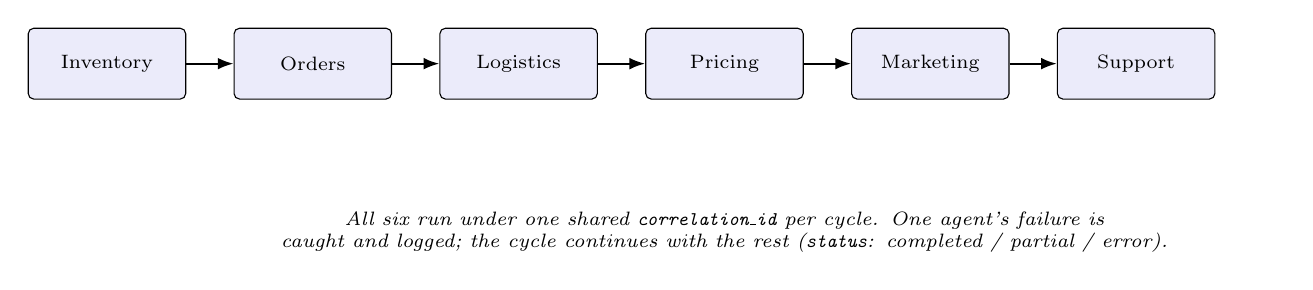
\begin{tikzpicture}[
  node distance=6mm,
  ag/.style={draw, rounded corners=2pt, fill=accent!12, minimum width=20mm, minimum height=9mm, align=center, font=\scriptsize, inner sep=2pt},
  arr/.style={-{Latex[length=2mm]}, thick}
]
\node[ag] (inv) {Inventory};
\node[ag, right=6mm of inv] (ord) {Orders};
\node[ag, right=6mm of ord] (log) {Logistics};
\node[ag, right=6mm of log] (pri) {Pricing};
\node[ag, right=6mm of pri] (mkt) {Marketing};
\node[ag, right=6mm of mkt] (sup) {Support};
\draw[arr] (inv) -- (ord); \draw[arr] (ord) -- (log); \draw[arr] (log) -- (pri);
\draw[arr] (pri) -- (mkt); \draw[arr] (mkt) -- (sup);
\node[below=13mm of pri, align=center, font=\scriptsize\itshape, text width=140mm] (note)
  {All six run under one shared \texttt{correlation\_id} per cycle. One agent's failure is\\
   caught and logged; the cycle continues with the rest (\texttt{status}: completed / partial / error).};
\end{tikzpicture}%
}
\caption{\texttt{orchestrator.py} -- a static pipeline, not a graph. This is the whole of \texttt{run\_orchestrator()}.}
\end{figure}

\begin{itemize}[itemsep=2pt]
  \item \texttt{orchestrator.py} holds a static \texttt{\_PIPELINE} list and calls each
  \texttt{run\_<name>\_agent(correlation\_id)} once, in the fixed order inventory $\to$ orders
  $\to$ logistics $\to$ pricing $\to$ marketing $\to$ support.
  \item Agents hand off work \textbf{through the database}, never directly: inventory writes
  purchase orders that pricing later reads as its cost basis; the order agent flips an order
  to \texttt{confirmed}, which the logistics agent then picks up to create a shipment.
  \item The \textbf{human hand-off} works the same way: an agent calls \texttt{enqueue\_review}
  which inserts a \texttt{review\_queue} row; a human resolves it on \texttt{/dashboard/review},
  which calls the server action \texttt{updateReviewStatus(...)} -- this cascades the decision
  into the right domain table (the PO, the price, the order, the refund, the campaign, the
  shipment) and stamps the reviewer's id and note.
  \item \texttt{correlation\_id} is a \textbf{grouping key}, not a channel -- it lets you look
  at \texttt{agent\_task\_log} or a Langfuse trace and see everything that happened in one
  cycle, but no agent ever reads another agent's \texttt{correlation\_id} to react to it.
  \item A \textbf{conflict guard} (\texttt{touched\_product\_ids}) is the one piece of real
  cross-agent signalling within a cycle: it is accumulated in memory as the pipeline runs and
  passed to marketing so it does not double-act on a SKU another agent already changed.
\end{itemize}

\begin{qabox}{Interview angle: ``why not a real multi-agent framework (LangGraph, CrewAI)?''}
Honest answer: for six agents with a fixed, known execution order and no need for dynamic
re-planning, a static pipeline plus shared Postgres state is simpler to debug, has zero extra
infrastructure, and every hand-off is auditable as ordinary rows in a table. A graph-based
orchestrator would earn its complexity if agents needed to dynamically decide \emph{who runs
next} based on results -- that is explicitly named as future work, not something avoided out
of ignorance.
\end{qabox}

% =====================================================================
\section{The Autopilot Ledger (Headline Feature)}
\label{sec:ledger}
% =====================================================================

This is the feature to lead with. Most ``agentic AI'' demos show an agent making a decision and
stop there -- there is no way to know if the decision was actually \emph{good}. The Autopilot
Ledger closes that loop for every judgement call the pricing, inventory, marketing, and support
agents make.

\subsection{How one decision is booked}
Every time an agent auto-executes or escalates a decision, it calls
\texttt{record\_action(...)} in \texttt{backend/agents/ledger.py}, which inserts one
\texttt{agent\_action} row containing:
\begin{enumerate}[itemsep=2pt]
  \item \textbf{The decision itself} -- e.g. \{old\_price, new\_price, effective\_cost\}.
  \item \textbf{A counterfactual baseline} -- the \Rs{} outcome of \emph{doing nothing},
  computed right now from data the agent already has (trailing sales velocity, margins, stock
  cover). The formula and every input value are stored in the row, so any number on the
  dashboard can be traced back to exactly how it was derived.
  \item \textbf{\texttt{verify\_after}} -- a settle window per action type, read from
  \texttt{store\_config} (e.g. 14 days for a price change, 7 + lead time for a purchase order,
  30 days for a refund).
\end{enumerate}

\begin{figure}[h]
\centering
\resizebox{\linewidth}{!}{%
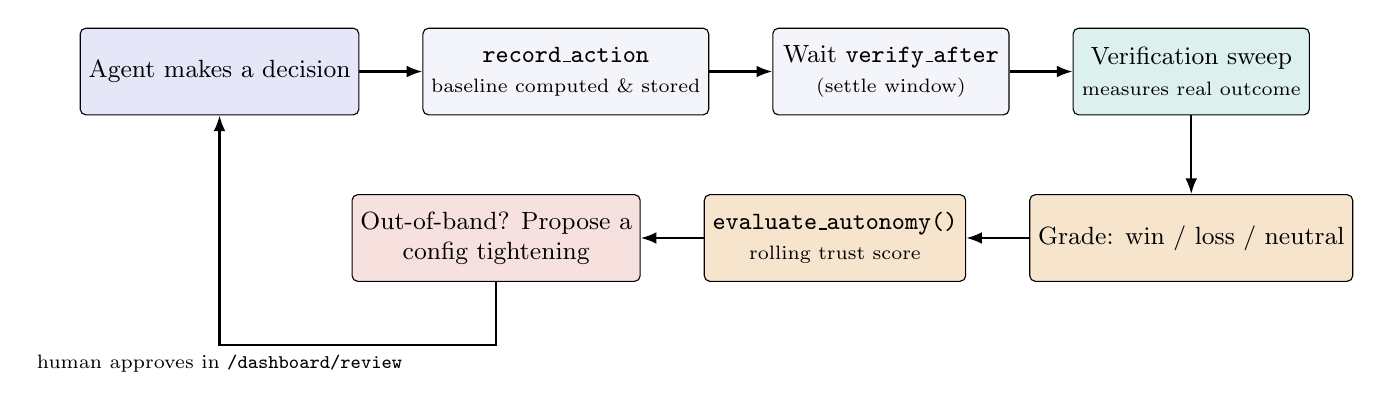
\begin{tikzpicture}[
  node distance=8mm and 8mm,
  st/.style={draw, rounded corners=2pt, fill=soft, minimum width=30mm, minimum height=11mm, align=center, font=\small, inner sep=3pt},
  arr/.style={-{Latex[length=2mm]}, thick}
]
\node[st, fill=accent!15] (dec) {Agent makes a decision};
\node[st, right=of dec] (base) {\texttt{record\_action}\\ \scriptsize baseline computed \& stored};
\node[st, right=of base] (wait) {Wait \texttt{verify\_after}\\ \scriptsize (settle window)};
\node[st, right=of wait, fill=accent2!15] (sweep) {Verification sweep\\ \scriptsize measures real outcome};
\node[st, below=10mm of sweep, fill=warn!20] (grade) {Grade: win / loss / neutral};
\node[st, left=of grade, fill=warn!20] (trust) {\texttt{evaluate\_autonomy()}\\ \scriptsize rolling trust score};
\node[st, left=of trust, fill=danger!15] (prop) {Out-of-band? Propose a\\ config tightening};
\draw[arr] (dec) -- (base); \draw[arr] (base) -- (wait); \draw[arr] (wait) -- (sweep);
\draw[arr] (sweep) -- (grade); \draw[arr] (grade) -- (trust); \draw[arr] (trust) -- (prop);
\draw[arr] (prop.south) |- ++(0,-8mm) -| node[below,font=\scriptsize]{human approves in \texttt{/dashboard/review}} (dec.south);
\end{tikzpicture}%
}
\caption{The Ledger's full lifecycle: decide $\to$ baseline $\to$ settle $\to$ verify $\to$ grade $\to$ trust score $\to$ (optionally) propose tightening the agent's own limits.}
\end{figure}

\subsection{Baseline formulas (the actual math)}
\begin{center}
\begin{tabular}{@{}p{2.6cm}p{9.6cm}@{}}
\toprule
\textbf{Action} & \textbf{Baseline (``do nothing'') formula} \\
\midrule
Price change & \texttt{daily\_velocity * settle\_days * (old\_price - effective\_cost)} -- the
margin dollars we'd have kept selling at the old price. \\
Purchase order & \texttt{-(max(0, velocity*lead\_days - available) * margin\_per\_unit)} -- the
margin we'd have \emph{lost} from stockouts if we hadn't reordered, net of a holding-cost
charge on the PO's value. \\
Campaign & \texttt{0} (no campaign = no lift); projected value is an assumed 1.5$\times$ ROAS
on budget -- explicitly labelled \emph{estimated}, not measured, because there's no real ESP. \\
Refund & \texttt{-support\_handle\_cost\_inr} -- the labour cost of escalating instead of
resolving now; also labelled \emph{estimated}. \\
\bottomrule
\end{tabular}
\end{center}

\subsection{Verification and Trust Score}
\begin{itemize}[itemsep=2pt]
\item \texttt{backend/agents/verification.py} \texttt{run\_verification\_sweep()} runs as a
second scheduled job (or on-demand via \texttt{POST /api/ledger/verify}). For every
\texttt{agent\_action} whose \texttt{verify\_after} has passed, it re-reads the operational
tables (actual sales, actual stock, actual refund status) to compute
\texttt{realized\_delta\_inr}, compares it to \texttt{baseline\_delta\_inr}, and grades the
decision \texttt{win} / \texttt{loss} / \texttt{neutral}.
\item \texttt{evaluate\_autonomy()} then looks at an agent's last
\texttt{ledger\_min\_sample} verified decisions. If the win-rate falls outside the
\texttt{[ledger\_win\_rate\_floor, ledger\_win\_rate\_ceiling]} band, it enqueues a
\texttt{review\_queue} item of type \texttt{autonomy\_adjustment} that proposes a
\textbf{concrete, one-click config change} (e.g. ``\texttt{budget\_auto\_approve\_limit}
200 $\to$ 120''), linked to the exact losing decisions that justify it.
\item Approving that proposal in \texttt{/dashboard/review} writes the new
\texttt{store\_config}/\texttt{agent\_config} value directly -- \textbf{the system tightens its
own leash based on evidence}, instead of a human guessing at a new threshold.
\item \texttt{/dashboard/ledger} shows, per agent: a \textbf{Trust Score}, realized
\Rs{} contribution (with a measured-vs-estimated split clearly labelled), and a
drill-down into every decision's stored baseline formula and actual outcome.
\end{itemize}

\subsection{Standing policies -- learning from human rejections}
When an operator rejects a review item, they can attach a one-line standing rule
(stored in \texttt{agent\_policy}). \texttt{base.py}'s \texttt{load\_active\_policies(agent\_name)}
prepends every active rule for that agent to its LLM system prompt on \emph{every future run} --
so ``don't discount SKU X below \Rs{}500'' said once keeps being obeyed.

\subsection{Fail-safe design}
\texttt{record\_action} is \textbf{best-effort}: any failure (including the Ledger tables not
existing yet, i.e. migration \texttt{016\_ledger.sql} not applied) is caught and logged, never
raised. The six agents run identically with or without the Ledger -- it observes, it never
gates.

% =====================================================================
\section{Database}
% =====================================================================

Supabase Postgres, 22 tables, all schema and seed data as plain numbered SQL migrations in
\texttt{database/migrations/} (\texttt{001}--\texttt{016}) -- no ORM, no migration framework
magic, just files run in order.

\begin{center}
\begin{tabular}{@{}p{3.6cm}p{9cm}@{}}
\toprule
\textbf{Migration} & \textbf{What it adds} \\
\midrule
001 & Extensions (\texttt{pgvector}) + a generic \texttt{updated\_at} trigger function \\
002--004 & Core schema: foundation tables, transactional tables (orders, order\_items,
purchase\_orders...), operational tables (inventory, shipments, tickets...) \\
005 & Seed data (demo store, users, products) \\
006 & Row-Level Security policies \\
007 & \texttt{notifications} table (dashboard feed) \\
008, 010, 014 & \texttt{agent\_config} reseeds / updates as tunables evolved \\
009 & Fixes broken \texttt{updated\_at} triggers \\
011 & Prunes seeded \texttt{agent\_task\_log} noise \\
012 & \texttt{match\_knowledge\_base} pgvector similarity RPC (support RAG) \\
013 & Agent RPCs: \texttt{apply\_price\_change}, \texttt{create\_po\_with\_review},
\texttt{confirm\_order\_and\_reserve} \\
015 & Pricing demo signal seed data \\
016 & \textbf{Autopilot Ledger}: \texttt{agent\_action}, \texttt{agent\_policy} tables +
\texttt{receive\_purchase\_order} / \texttt{release\_order\_reservation} RPCs \\
\bottomrule
\end{tabular}
\end{center}

\textbf{Why RPCs (stored procedures) for the risky writes:} \texttt{apply\_price\_change},
\texttt{confirm\_order\_and\_reserve}, and \texttt{receive\_purchase\_order} all touch two or
more tables that must stay consistent (e.g. reserve stock \emph{and} confirm the order, or
nothing). Doing that as a single Postgres function call makes it one atomic transaction instead
of two separate round-trips from Python that could interleave with another request.

% =====================================================================
\section{APIs}
% =====================================================================

There are two API surfaces, deliberately kept thin.

\subsection{FastAPI (\texttt{backend/}) -- does the real work}
\begin{center}
\begin{tabular}{@{}p{1.2cm}p{4.6cm}p{6.8cm}@{}}
\toprule
\textbf{Method} & \textbf{Path} & \textbf{Purpose} \\
\midrule
GET & \texttt{/}, \texttt{/health} & Liveness check \\
POST & \texttt{/api/auth/login} & Verifies bcrypt/SHA1 password, 5-per-15-min rate limit per
email+IP. Returns the user; \textbf{does not} issue a token -- the web layer signs the session. \\
POST & \texttt{/api/auth/change-password} & Re-verifies current password before writing a new
bcrypt hash \\
POST & \texttt{/api/agents/\{agent\_name\}/run} & Runs one agent or the orchestrator; returns
\{status, log\_id, correlation\_id, summary: \{scanned, auto\_executed, escalated\}\} \\
GET & \texttt{/api/agents/scheduler} & \{enabled, running, interval\_minutes, last\_cycle\_at,
last\_cycle\_status\} for the ``Autonomous mode'' badge \\
POST & \texttt{/api/simulate/orders} & Inserts realistic synthetic orders (\texttt{?count},
\texttt{?trigger\_agents}) -- this is how demo data flows in, since there is no real storefront \\
GET & \texttt{/api/ledger/summary} & Ledger report cards per agent: wins/losses, realized
\Rs{}, trust score \\
GET & \texttt{/api/ledger/actions} & Raw \texttt{agent\_action} rows for the drill-down table \\
POST & \texttt{/api/ledger/verify} & Runs the verification sweep on demand \\
\bottomrule
\end{tabular}
\end{center}
Interactive Swagger docs are served live at \texttt{/docs} (and ReDoc at \texttt{/redoc}) --
worth opening in a live demo.

\subsection{Next.js route handlers (\texttt{apps/web/app/api/}) -- thin auth-gated proxies}
Every route here does one job: check the \texttt{trucart\_session} cookie (via
\texttt{middleware.ts}), then forward the request to FastAPI. \texttt{/api/auth/login} is the
one exception -- on a successful FastAPI response it \emph{signs} the HS256 session cookie
(8-hour expiry, httpOnly). \texttt{/api/auth/logout} just clears it.

\subsection{Server actions -- not REST at all}
Most dashboard mutations (updating a review, changing a config value, editing a profile) never
go through an HTTP API. They are Next.js \textbf{server actions} defined in
\texttt{apps/web/app/dashboard/actions.ts}, called directly from React components, running on
the server with the Supabase service-role client. The most important one,
\texttt{updateReviewStatus(reviewId, status, \{note, makeStandingRule\})}, resolves the reviewer
from the verified session, cascades the approval into the right domain table, and (if the item
is an \texttt{autonomy\_adjustment}) writes the proposed config change.

\begin{qabox}{Interview angle: ``REST API vs. server actions -- why both?''}
Server actions exist because the dashboard reads/writes are same-origin, same-request
mutations triggered from a form or button -- a full REST round trip would just be overhead.
The FastAPI surface exists because agent execution is genuinely a different service (Python,
long-running LLM calls, its own deploy target) that the Next.js app must call over the network.
Using server actions everywhere would have meant putting agent logic inside Next.js; keeping
FastAPI separate keeps the Python ML/agent code independently deployable and testable.
\end{qabox}

% =====================================================================
\section{Frontend / Dashboard}
% =====================================================================

Next.js 16 App Router, React 19 Server Components, Tailwind v4, and a shared \texttt{shadcn/ui}
component package (\texttt{packages/ui}) used by both \texttt{apps/web} and any future app in
the monorepo. Screens live one-per-folder under \texttt{apps/web/app/dashboard/}:

\begin{center}
\begin{tabular}{@{}ll@{}}
\toprule
\textbf{Route} & \textbf{What it shows} \\
\midrule
\texttt{/dashboard} & Overview -- KPIs, recent activity \\
\texttt{/dashboard/agents} & Run agents on-demand, Configure knobs, Autonomous-mode badge \\
\texttt{/dashboard/orders} & Order list, ``Simulate incoming orders'' button \\
\texttt{/dashboard/inventory} & Stock levels, purchase orders \\
\texttt{/dashboard/logistics} & Shipment lifecycle tracking \\
\texttt{/dashboard/pricing} & Price history, current margins \\
\texttt{/dashboard/marketing} & Campaigns \\
\texttt{/dashboard/support} & Ticket queue \\
\texttt{/dashboard/review} & Human review queue -- approve/reject every escalation \\
\texttt{/dashboard/ledger} & \textbf{Autopilot Ledger} -- trust scores, realized \Rs{}, drill-down \\
\texttt{/dashboard/audits} & \texttt{agent\_task\_log} history per cycle \\
\texttt{/dashboard/notifications} & Live notification feed \\
\texttt{/dashboard/settings} & Profile, password, account deactivation \\
\bottomrule
\end{tabular}
\end{center}

\textbf{Pattern used throughout:} each screen is a pair of files -- \texttt{page.tsx} is a
Server Component that fetches data directly from Supabase (no client-side loading spinners for
the initial view) and \texttt{*-client.tsx} holds the interactive parts (tables with filters,
buttons that call server actions). This keeps data fetching co-located with rendering and
avoids waterfalls of client-side \texttt{fetch} calls.

% =====================================================================
\section{Authentication \& Security}
% =====================================================================

\begin{itemize}[itemsep=2pt]
\item Single staff role model (\texttt{users.role = 'admin'}) -- this is an internal ops tool,
not a customer-facing app, so there is no signup flow or multi-tenant RBAC.
\item \textbf{Login flow:} browser $\to$ Next.js \texttt{/api/auth/login} $\to$ FastAPI
verifies the password hash (bcrypt, with a legacy SHA1 path) and applies an in-memory rate
limit (5 attempts / 15 minutes per email+IP) $\to$ on success, the \textbf{Next.js layer}
signs an 8-hour HS256 JWT into an httpOnly \texttt{trucart\_session} cookie. FastAPI itself
never issues a token.
\item \texttt{middleware.ts} verifies that cookie on every request to \texttt{/dashboard/*},
\texttt{/api/agents/*}, and \texttt{/api/simulate/*}; unauthenticated API calls get 401, pages
redirect to \texttt{/login}.
\item The cookie is only marked \texttt{Secure} when the request actually arrived over HTTPS
(checked via \texttt{x-forwarded-proto}) -- a small but important detail that lets login work
over plain HTTP on an EC2 demo box without a TLS-terminating proxy in front, without weakening
security on a real HTTPS deployment.
\item FastAPI holds the Supabase \textbf{service-role} key (bypasses Row-Level Security) --
by design it must sit behind the Next.js/Vercel proxy and never be exposed directly to the
public internet in a real deployment.
\item Account management: \texttt{POST /api/auth/change-password} re-verifies the current
password; \texttt{deactivateAccount} sets \texttt{users.is\_active = false}.
\item Known gaps, stated openly: no signup, no MFA, no server-side session revocation list
(the JWT is valid until it expires, full stop).
\end{itemize}

% =====================================================================
\section{Docker \& Deployment}
% =====================================================================

\subsection{Two containers}
\begin{center}
\begin{tabular}{@{}p{3.4cm}p{9.4cm}@{}}
\toprule
\textbf{Image} & \textbf{How it's built} \\
\midrule
\texttt{backend/Dockerfile} & \texttt{python:3.12-slim} $\to$ installs build tools (for
\texttt{bcrypt}'s native extension) $\to$ \texttt{pip install -r requirements.txt} $\to$ copies
\texttt{backend/} $\to$ runs \texttt{uvicorn backend.main:app} on port 8000. \\
\texttt{apps/web/Dockerfile} & Multi-stage: \texttt{deps} (installs npm workspace deps),
\texttt{builder} (bakes \texttt{NEXT\_PUBLIC\_API\_URL} and \texttt{SESSION\_SECRET} as build
args, runs \texttt{next build} with Next's \emph{standalone} output), \texttt{runner}
(non-root \texttt{nextjs} user, copies only the standalone bundle + static assets, runs
\texttt{node server.js} on port 3000). \\
\bottomrule
\end{tabular}
\end{center}
Prebuilt images are published to Docker Hub as \texttt{bhautik2004/trucart-backend} and
\texttt{bhautik2004/trucart-web}.

\subsection{Two compose files, two purposes}
\begin{itemize}[itemsep=2pt]
\item \textbf{\texttt{docker-compose.yml}} (local dev) -- \textbf{builds} both images from
source, wires \texttt{web}'s \texttt{NEXT\_PUBLIC\_API\_URL} build-arg to
\texttt{http://backend:8000} (the Docker-internal service name, not \texttt{localhost}, because
the variable gets baked into client-shipped JS at build time), exposes web on port 80 and
backend on 8000.
\item \textbf{\texttt{docker-compose.prod.yml}} (deployment) -- \textbf{pulls} the prebuilt
Docker Hub images instead of building on the target machine. This matters concretely: a
\texttt{t2.micro} EC2 instance (1 vCPU / 1 GB RAM) cannot reliably run \texttt{next build}, but
running the two already-built containers fits comfortably (roughly 150 MB combined).
\end{itemize}

\subsection{AWS EC2 deployment (the live demo)}
\begin{enumerate}[itemsep=2pt]
\item Launch a \texttt{t2.micro}/\texttt{t3.micro} instance (Amazon Linux 2023, free tier),
using \texttt{deploy/ec2-bootstrap.sh} as the instance \emph{User data} script -- it installs
Docker + Compose and clones the repo automatically at boot.
\item Open inbound ports 80 (dashboard) and 8000 (API) in the security group.
\item Write real secrets into \texttt{\textasciitilde/TruCart/.env.local} on the instance
(Supabase keys, an LLM API key, a real \texttt{SESSION\_SECRET}), plus
\texttt{CORS\_ALLOW\_ORIGINS=http://<EC2-PUBLIC-IP>}.
\item \texttt{docker compose -f docker-compose.prod.yml --env-file .env.local pull \&\& up -d}.
\end{enumerate}
\textbf{To ship a code change}: rebuild + push the image(s) \emph{locally}, then on the
instance just re-run \texttt{pull \&\& up -d} -- no build ever happens on the tiny instance
itself. On the live box, \texttt{OLLAMA\_BASE\_URL} is pointed at Groq's OpenAI-compatible
endpoint (a free hosted LLM) instead of a local Ollama server, since a 7B model won't fit in
1\,GB of RAM.

% =====================================================================
\section{CI Pipeline}
% =====================================================================

\texttt{.github/workflows/ci.yml} runs on every push to \texttt{main} and every pull request,
as two independent jobs on \texttt{ubuntu-latest}:

\begin{center}
\begin{tabular}{@{}p{2.4cm}p{9.6cm}@{}}
\toprule
\textbf{Job} & \textbf{Steps} \\
\midrule
\texttt{backend} & Checkout $\to$ set up Python 3.12 $\to$
\texttt{pip install -r backend/requirements-dev.txt} $\to$
\texttt{python -m pytest backend/tests -q} \\
\texttt{web} & Checkout $\to$ set up Node 20 (npm cache) $\to$ \texttt{npm ci} $\to$
\texttt{npx turbo lint typecheck build --filter=web --filter=@workspace/ui} (with a
placeholder \texttt{SESSION\_SECRET} so the build doesn't fail on the startup guard) \\
\bottomrule
\end{tabular}
\end{center}

This is intentionally a \textbf{quality gate, not a deploy pipeline} -- there is no CD step;
deployment is the manual Docker Hub push + EC2 pull described above. Turborepo's
\texttt{--filter} flags mean only the \texttt{web} app and the shared \texttt{ui} package are
linted/typechecked/built (the two packages that matter for a passing frontend build), keyed to
Turborepo's own dependency graph.

\begin{qabox}{Interview angle: ``why no CD / auto-deploy?''}
Time-boxed hackathon scope: a manual two-command deploy (\texttt{pull \&\& up -d}) to a single
EC2 box is proportionate to a single-environment demo. The natural next step named in the docs
is a GitHub Actions job that builds \& pushes the Docker images on merge to \texttt{main}, and
optionally SSHes into the instance to pull -- straightforward to add on top of the existing
Dockerfiles without changing them.
\end{qabox}

% =====================================================================
\section{LLM Integration \& Observability}
% =====================================================================

\begin{itemize}[itemsep=2pt]
\item All agents talk to the LLM through one function: \texttt{call\_llm\_json(system\_prompt,
user\_prompt, ...)} in \texttt{base.py}. It always asks for
\texttt{response\_format=\{"type": "json\_object"\}} at low temperature (0.2), parses the
result, and returns \texttt{None} on \emph{any} failure -- malformed JSON, network error,
timeout -- so the calling agent can fall back to a deterministic rule instead of crashing.
\item The client is pointed at an OpenAI-compatible base URL (\texttt{OLLAMA\_BASE\_URL}),
which is why the same code path works against local Ollama, Groq, or OpenRouter -- just swap
the base URL, model name, and API key.
\item \textbf{Langfuse} is wired in as a drop-in replacement for the OpenAI client
(\texttt{langfuse.openai}) when its keys are configured -- every chat completion is
automatically captured as a trace with model, token usage, latency, and errors, with
\emph{zero} manual span code in the agents themselves. Each trace's id is deterministically
derived from the same \texttt{correlation\_id} already written to \texttt{agent\_task\_log},
so a Supabase row and a Langfuse trace can be cross-referenced by one id.
\item Tracing is \textbf{fully best-effort}: if Langfuse keys are missing or its SDK throws
during setup, tracing is silently and permanently disabled for the rest of the process, and
the underlying LLM call still happens normally.
\item Token usage per agent run is accumulated across every LLM call an agent makes during one
correlation\_id, then drained into the single \texttt{agent\_task\_log.tokens\_used} column
when that agent finishes -- so ``run full cycle'' shows one token count per agent, not one per
LLM call.
\end{itemize}

% =====================================================================
\section{Autonomy Modes}
% =====================================================================

\begin{itemize}[itemsep=2pt]
\item \textbf{Manual:} ``Run Agent'' / ``Run full cycle'' buttons on \texttt{/dashboard/agents}
call the route handler, which calls the FastAPI runner directly.
\item \textbf{Scheduled:} \texttt{backend/scheduler.py} starts an APScheduler
\texttt{BackgroundScheduler} when \texttt{SCHEDULER\_ENABLED=true}, running
\texttt{run\_orchestrator} every \texttt{ORCHESTRATOR\_INTERVAL\_MINUTES} (default 10). This
is literally what ``autonomous'' means in this build -- a timer, not event-driven triggering.
\item A \textbf{second} scheduled job runs the Ledger's verification sweep independently of
the main pipeline.
\item Every runner is \textbf{idempotent}: it skips items already queued, POs already open, or
products with a too-recent price change, and is bounded by \texttt{max\_items\_per\_run} --
so running the same cycle twice in a row (or the scheduler firing while a manual run is still
warm) never double-executes anything.
\end{itemize}

% =====================================================================
\section{Scope \& Honest Limitations}
\label{sec:limits}
% =====================================================================

Stated openly in the README -- know these cold, because an interviewer probing depth will ask
about them and the strongest answer is to name the simplification \emph{before} they do.

\begin{keybox}
\begin{itemize}[itemsep=2pt]
\item \textbf{No real storefront.} Orders arrive via \texttt{POST /api/simulate/orders} --
there's no checkout, payment gateway, or fraud check to integrate with.
\item \textbf{No carrier API.} Logistics invents carrier/tracking/cost and advances shipments
on a timer, not real carrier webhooks.
\item \textbf{Inventory reorders a fixed quantity} -- not demand-forecasted; it does receive
POs and increment stock, but does not update \texttt{cost\_price} on receipt.
\item \textbf{Marketing overstock detection is a coarse ratio test}, and ``sending'' a campaign
just inserts a row -- no ESP, fabricated metrics.
\item \textbf{Support refunds are whole-order only}, no payment gateway, no partial refund/RMA.
\item \textbf{No outbound customer comms} -- the notification feed is internal-only.
\item \textbf{Ledger's marketing/support baselines are modelled, not measured} -- clearly
labelled ``estimated'' wherever shown, versus pricing/inventory which use real operational
data (``measured'').
\item \textbf{RAG needs a one-off embedding backfill} (\texttt{npm run seed:rag}) before the
support agent has any knowledge-base context; without it, it triages blind.
\item \textbf{Auth has no MFA, no signup, no session revocation store.}
\end{itemize}
\end{keybox}

The large AWS/Bedrock/LangGraph design in \texttt{ai-ecommerce-platform-plan.md} is the
\emph{funded production target}, explicitly documented as \textbf{not} what runs here --
everything in this report is what is deployable on free tiers today.

% =====================================================================
\section{Interview Q\&A Cheat Sheet}
% =====================================================================

\begin{qabox}{``Walk me through what happens when the scheduler fires.''}
APScheduler calls \texttt{run\_orchestrator()} with a fresh \texttt{correlation\_id}. It runs
inventory, then orders, then logistics, then pricing, then marketing, then support, each
writing its own \texttt{agent\_task\_log} row under that id. Each agent loads its config,
scans its slice of the DB, optionally asks the LLM for a judgement call, clamps that with
guardrails, executes safe actions immediately via RPCs, and enqueues anything risky to
\texttt{review\_queue} (which also creates a dashboard notification). Every judgement-call
decision (pricing/inventory/marketing/support) also gets booked into the Autopilot Ledger with
a baseline. If any one agent throws, it's caught, logged as an error for that agent, and the
rest of the pipeline still runs.
\end{qabox}

\begin{qabox}{``How do you prevent the LLM from doing something dangerous?''}
The LLM never executes anything directly -- it only returns a JSON opinion (e.g. target price,
raise/reduce/hold, urgency). Python code then clamps that opinion against deterministic
guardrails computed independently of the LLM: a price can never go below unit cost or move more
than 15\% in one step; a refund can never exceed the order total or auto-approve above \Rs{}100; a
purchase order over \Rs{}5,000 always needs a human. If the LLM is unreachable or returns garbage,
\texttt{call\_llm\_json} returns \texttt{None} and the agent falls back to a pure rule-based
decision (usually: escalate).
\end{qabox}

\begin{qabox}{``What's the hardest technical problem you solved?''}
Making the reservation/confirmation path race-safe without a lock service: two orders for the
same last unit of stock must not both succeed. Solved with the \texttt{confirm\_order\_and\_reserve}
Postgres RPC -- a single atomic transaction that checks availability and reserves stock in one
statement, so Postgres's own transaction isolation does the concurrency control instead of
application-level locking.
\end{qabox}

\begin{qabox}{``How do you know the agents are actually helping, not just automating noise?''}
That's exactly what the Autopilot Ledger measures. Every decision is booked against a
computed counterfactual baseline at decision time, then graded weeks later against what
actually happened. The per-agent trust score and realized-\Rs{} numbers on \texttt{/dashboard/ledger}
come directly from that, and if an agent's win-rate falls outside an acceptable band the system
proposes tightening its own auto-approve limit -- with the losing decisions attached as
evidence -- rather than a human guessing.
\end{qabox}

\begin{qabox}{``Why FastAPI + Next.js instead of one framework end to end?''}
The agent/orchestrator logic is Python because that's where the LLM/data-science ecosystem
lives and because it needed to be independently deployable/scalable/schedulable (APScheduler)
from the web tier. The dashboard is Next.js because Server Components let most screens fetch
directly from Supabase with zero client-side loading state, and \texttt{shadcn/ui} gives a fast,
consistent component set. The two talk over a small, explicit REST surface plus a session
cookie -- not tightly coupled, easy to reason about, easy to deploy separately (Vercel + any
Python host).
\end{qabox}

\begin{qabox}{``What would you build next if you had more time?''}
In order of value: (1) event-driven triggering instead of a fixed timer (DB triggers/webhooks
so agents react within seconds, not up to 10 minutes); (2) demand-forecasted reorder quantities
instead of a fixed number; (3) a real ESP and carrier API integration behind the same
guardrail pattern already in place; (4) partial refunds/RMA; (5) a CD step that builds and
pushes the Docker images automatically on merge to \texttt{main}.
\end{qabox}

\vspace{1cm}
\begin{center}
\small\textcolor{gray}{Generated as an interview preparation reference from the TruCart codebase.\\
Source: \texttt{docs/}, \texttt{README.md}, \texttt{backend/agents/}, \texttt{apps/web/}, \texttt{.github/workflows/ci.yml}.}
\end{center}

\end{document}
